\documentclass[convert={outext=.svg}]{standalone}
\usepackage{tikz}
\begin{document}

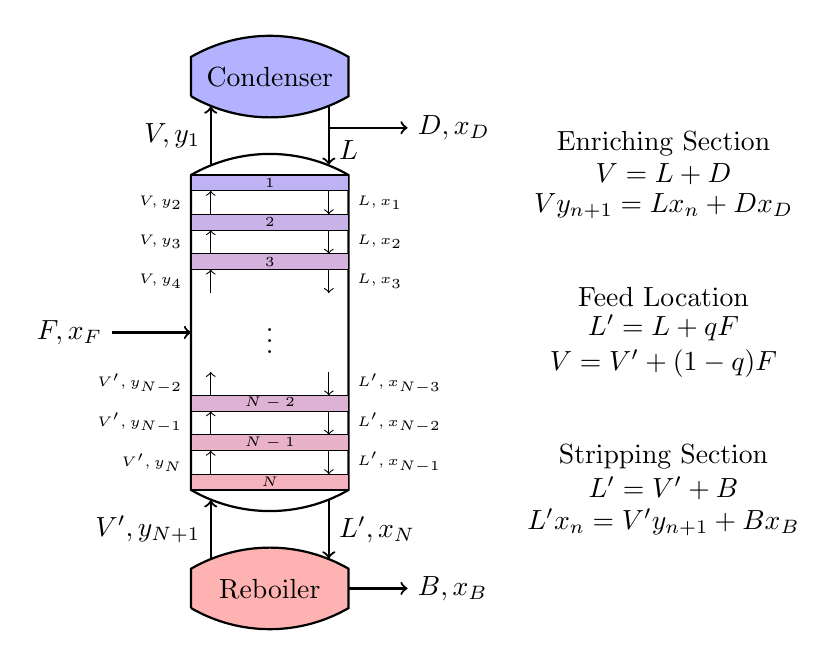
\begin{tikzpicture}
  %\draw[step=1cm,gray,very thin] (0,0) grid (10,8);
  
  % column outline
  \draw [thick] (2,2) arc (240:300:2cm) -- ++(0,4) arc (60:120:2cm) -- ++(0,-4);
  \draw [<-,thick] (2,4) -- ++(-1,0) node [left] {$F, x_F$};
  \draw (3,4) node {$\vdots$};
  
  % condensor
  \draw [thick,fill=blue!30] (2,7) arc (240:300:2cm) -- ++(0,0.5) arc (60:120:2cm) -- ++(0,-0.5);
  \draw (3,7.25) node {Condenser};
  \draw [->,thick] (2.25,6.13) -- ++(0,0.74) node[midway,left] {$V, y_1$};
  \draw [<-,thick] (3.75,6.13) -- ++(0,0.37) node[midway,right] {$L$} -- ++(0,0.37);
  \draw [->,thick] (3.75,6.6) -- ++(1,0) node [right] {$D, x_D$};
  
  % reboiler
  \draw [thick,fill=red!30] (2,0.5) arc (240:300:2cm) -- ++(0,0.5) arc (60:120:2cm) -- ++(0,-0.5);
  \draw (3,0.75) node {Reboiler};
  \draw [->,thick] (2.25,1.13) -- ++(0,0.74) node[midway,left] {$V', y_{N+1}$};
  \draw [<-,thick] (3.75,1.13) -- ++(0,0.74) node[midway,right] {$L', x_N$};
  \draw [->,thick] (4,0.75) -- ++(0.75,0) node [right] {$B, x_B$};
  
  % enriching section
  \draw [fill=red!15!blue!30,thin] (2,5.8) -- ++(2,0) -- ++(0,0.2) -- ++(-2,0) -- ++(0,-0.2);
    \draw (3,5.9) node {\tiny $1$};
    \draw [<-] (2.25,5.8) -- ++(0,-.3) node[midway,left] {\tiny $V, y_2 \quad$};
    \draw [->] (3.75,5.8) -- ++(0,-.3) node[midway,right] {\tiny\quad $L, x_1$};
  \draw [fill=red!30!blue!30,thin] (2,5.3) -- ++(2,0) -- ++(0,0.2) -- ++(-2,0) -- ++(0,-0.2);
    \draw (3,5.4) node {\tiny $2$};
    \draw [<-] (2.25,5.3) -- ++(0,-.3) node[midway,left] {\tiny $V, y_3 \quad$};
    \draw [->] (3.75,5.3) -- ++(0,-.3) node[midway,right] {\tiny\quad $L, x_2$};
  \draw [fill=red!45!blue!30,thin] (2,4.8) -- ++(2,0) -- ++(0,0.2) -- ++(-2,0) -- ++(0,-0.2);
    \draw (3,4.9) node {\tiny $3$};
    \draw [<-] (2.25,4.8) -- ++(0,-.3) node[midway,left] {\tiny $V, y_4 \quad$};
    \draw [->] (3.75,4.8) -- ++(0,-.3) node[midway,right] {\tiny\quad $L, x_3$};
  
  % stripping section
  \draw [fill=blue!15!red!30,thin] (2,2.2) -- ++(2,0) -- ++(0,-0.2) -- ++(-2,0) -- ++(0,+0.2);
    \draw (3,2.1) node {\tiny $N$};
    \draw [->] (2.25,2.2) -- ++(0,+0.3) node[midway,left] {\tiny $V', y_N \quad$};
    \draw [<-] (3.75,2.2) -- ++(0,+0.3) node[midway,right] {\tiny $\quad L', x_{N-1}$};
  \draw [fill=blue!30!red!30,thin] (2,2.7) -- ++(2,0) -- ++(0,-0.2) -- ++(-2,0) -- ++(0,+0.2);
    \draw (3,2.6) node {\tiny $N-1$};
    \draw [->] (2.25,2.7) -- ++(0,+0.3) node[midway,left] {\tiny $V', y_{N-1} \quad$};
    \draw [<-] (3.75,2.7) -- ++(0,+0.3) node[midway,right] {\tiny $\quad L', x_{N-2}$};
  \draw [fill=blue!45!red!30,thin] (2,3.2) -- ++(2,0) -- ++(0,-0.2) -- ++(-2,0) -- ++(0,+0.2);
    \draw (3,3.1) node {\tiny $N-2$};
    \draw [->] (2.25,3.2) -- ++(0,+0.3) node[midway,left] {\tiny $V', y_{N-2} \quad$};
    \draw [<-] (3.75,3.2) -- ++(0,+0.3) node[midway,right] {\tiny $\quad L', x_{N-3}$};
  
  % Model Equations
  \draw (8,6) node {\shortstack{Enriching Section \\ $V = L + D$ \\ $Vy_{n+1} = Lx_n + Dx_D$}};
  \draw (8,4) node {\shortstack{Feed Location \\ $L' = L + qF$ \\ $V = V' + (1-q)F$}};
  \draw (8,2) node {\shortstack{Stripping Section \\ $L' = V' + B$ \\ $L'x_n = V'y_{n+1} + Bx_B$}};

\end{tikzpicture}

\end{document}